\documentclass[xcolor=dvipsnames,t]{beamer}
%\beamertemplatenavigationsymbolsempty

%%\usepackage{enumitem}


\usepackage{svg}
\usepackage{graphicx}
\usepackage{outlines}
\usepackage{comment}
\usepackage{fourier}
\newcommand\fixmegood[1]{\textcolor{red}{#1}}



\graphicspath {{.}}

%\mode<presentation>
{
\usetheme{Warsaw}
%\usetheme{CambridgeUS}
%\usetheme{Madrid}
%\usetheme{Luebeck}
%\useoutertheme[subsection=false]{miniframes}

\useoutertheme{infolines}

%\useoutertheme{default}

%\useoutertheme{split}



% Circles in plain color (no 3D effect).
\useinnertheme{circles}

\definecolor{NiceBlue}{rgb}{0.04,0.13,0.26}

% Define corporate color
\definecolor{Corporate}{RGB}{228,102,10}
%\usecolortheme[named=Corporate]{structure}

  % or ...
  %\setbeamercovered{transparent}
  % or whatever (possibly just delete it)
%}

\usepackage[english]{babel}
\usepackage[utf8]{inputenc}

\title {Just enough SysML}
\subtitle {Concepts on SysML modelling of structure and behaviour}
\author[Jose A. Esparza Isasa (jois)]{{Jos\'e Antonio Esparza Isasa}\newline\url{jois@demant.com} }
%%\date {\today}

\date[] % (optional, should be abbreviation of conference name)
{Knowledge sharing session @ HWAS \newline Kongebakken, September 2023}

\begin {document}

\begin{frame} %[plain]
\vspace{1cm}
\titlepage
%\logo{\includegraphics[height=1cm]{i2.png}
%  \hspace{4.2 in}
%    \includegraphics[height=1cm]{i3.png}}
\begin{center}
%%%%%%%%%%%%%%%%%%%\includegraphics[height=1cm]{OMlogo.png}
\end{center}
\end{frame}


\begin{frame}{Agenda}
 \tableofcontents
  % You might wish to add the option [pausesections]
  % To keep a specific subsection out of the index use: \subsection*{...}
  % To remove all subsections from the TOC only, use: \tableofcontents[hideallsubsections]

%% Appendix A:\\
%% Appendix B:\\
%% Appendix C:
\end{frame}


\section{Introduction and overview of SysML}

%\begin{frame}
%\frametitle {The System Modelling Language (SysML)}
%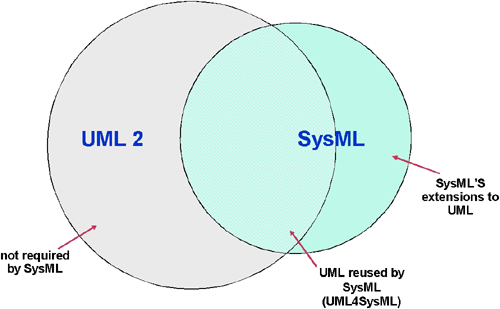
\includegraphics[width=0.5\textwidth]{SysMLsuperset.jpg}
%\end{frame}

\subsection{Overview of SysML}
\begin{frame}
\frametitle {The System Modelling Language (SysML)}
\vspace{-0.5cm}
     \begin{columns}
    \begin{column}{0.55\textwidth}
\vspace{0.5cm}
        \begin{itemize}
            \item It is a general purpose modelling language for systems engineering.
            \item INCOSE started developing it in 2001. Current version is 1.6 and version 2 should be released next year.

         \end{itemize}
     \end{column}
     
    \begin{column}{0.45\textwidth}
        \begin{figure}
            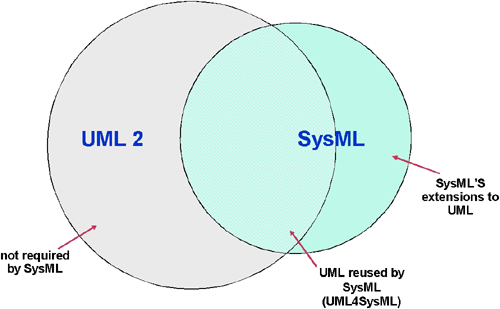
\includegraphics[width=.9\textwidth]{SysMLsuperset.jpg}
            %\caption{}
	\end{figure}
     \end{column}
     \end{columns}

\vspace{0.5cm}
\begin{itemize}
            \item Partially reuses UML2, and defines new elements. Biased by software abstractions in some aspects.
            \item It is a language, that has a syntax, and models have semantics.
            \item Syntactical correctness does not imply semantical correctness.
\end{itemize}
\vspace{0.5cm}
For some, the \textit{Characteristica Universalis} in systems engineering (more if we have time).
\end{frame} 

\begin{frame}
\frametitle {SysML Diagram Taxonomy}
%%\vspace{2cm}
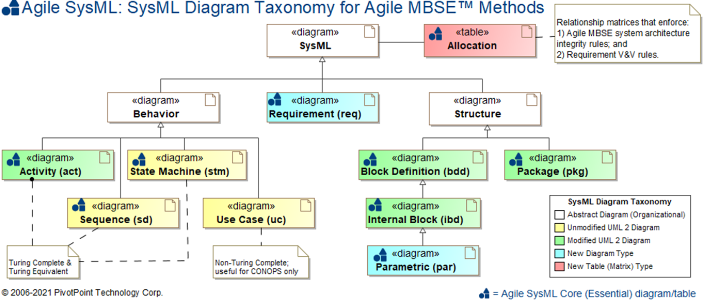
\includegraphics[width=\textwidth]{DiagramTaxonomy.png}
\begin{itemize}
\item Four diagrams to represent behaviour and four for structure.
\item State machines, BDDs and IBDs are the most relevant in DeviceHW.
\item Parametric and Requirement diagrams are not that relevant.
\end{itemize}
\end{frame}

\subsection{\textit{Mini} case study}
\begin{frame}
\frametitle {\textit{Mini} case study: quadcopter for nuclear emergencies (I/II)}
%% \begin{block}{} \end{block}
\begin{itemize}
\item A \href{https://en.wikipedia.org/wiki/Quadcopter}{quadcopter} for visual inspection and radiation monitoring.
\item Why not a Hearing Aid or an accessory? To avoid discussing very specific technical details rather than the language or the models.
\end{itemize}

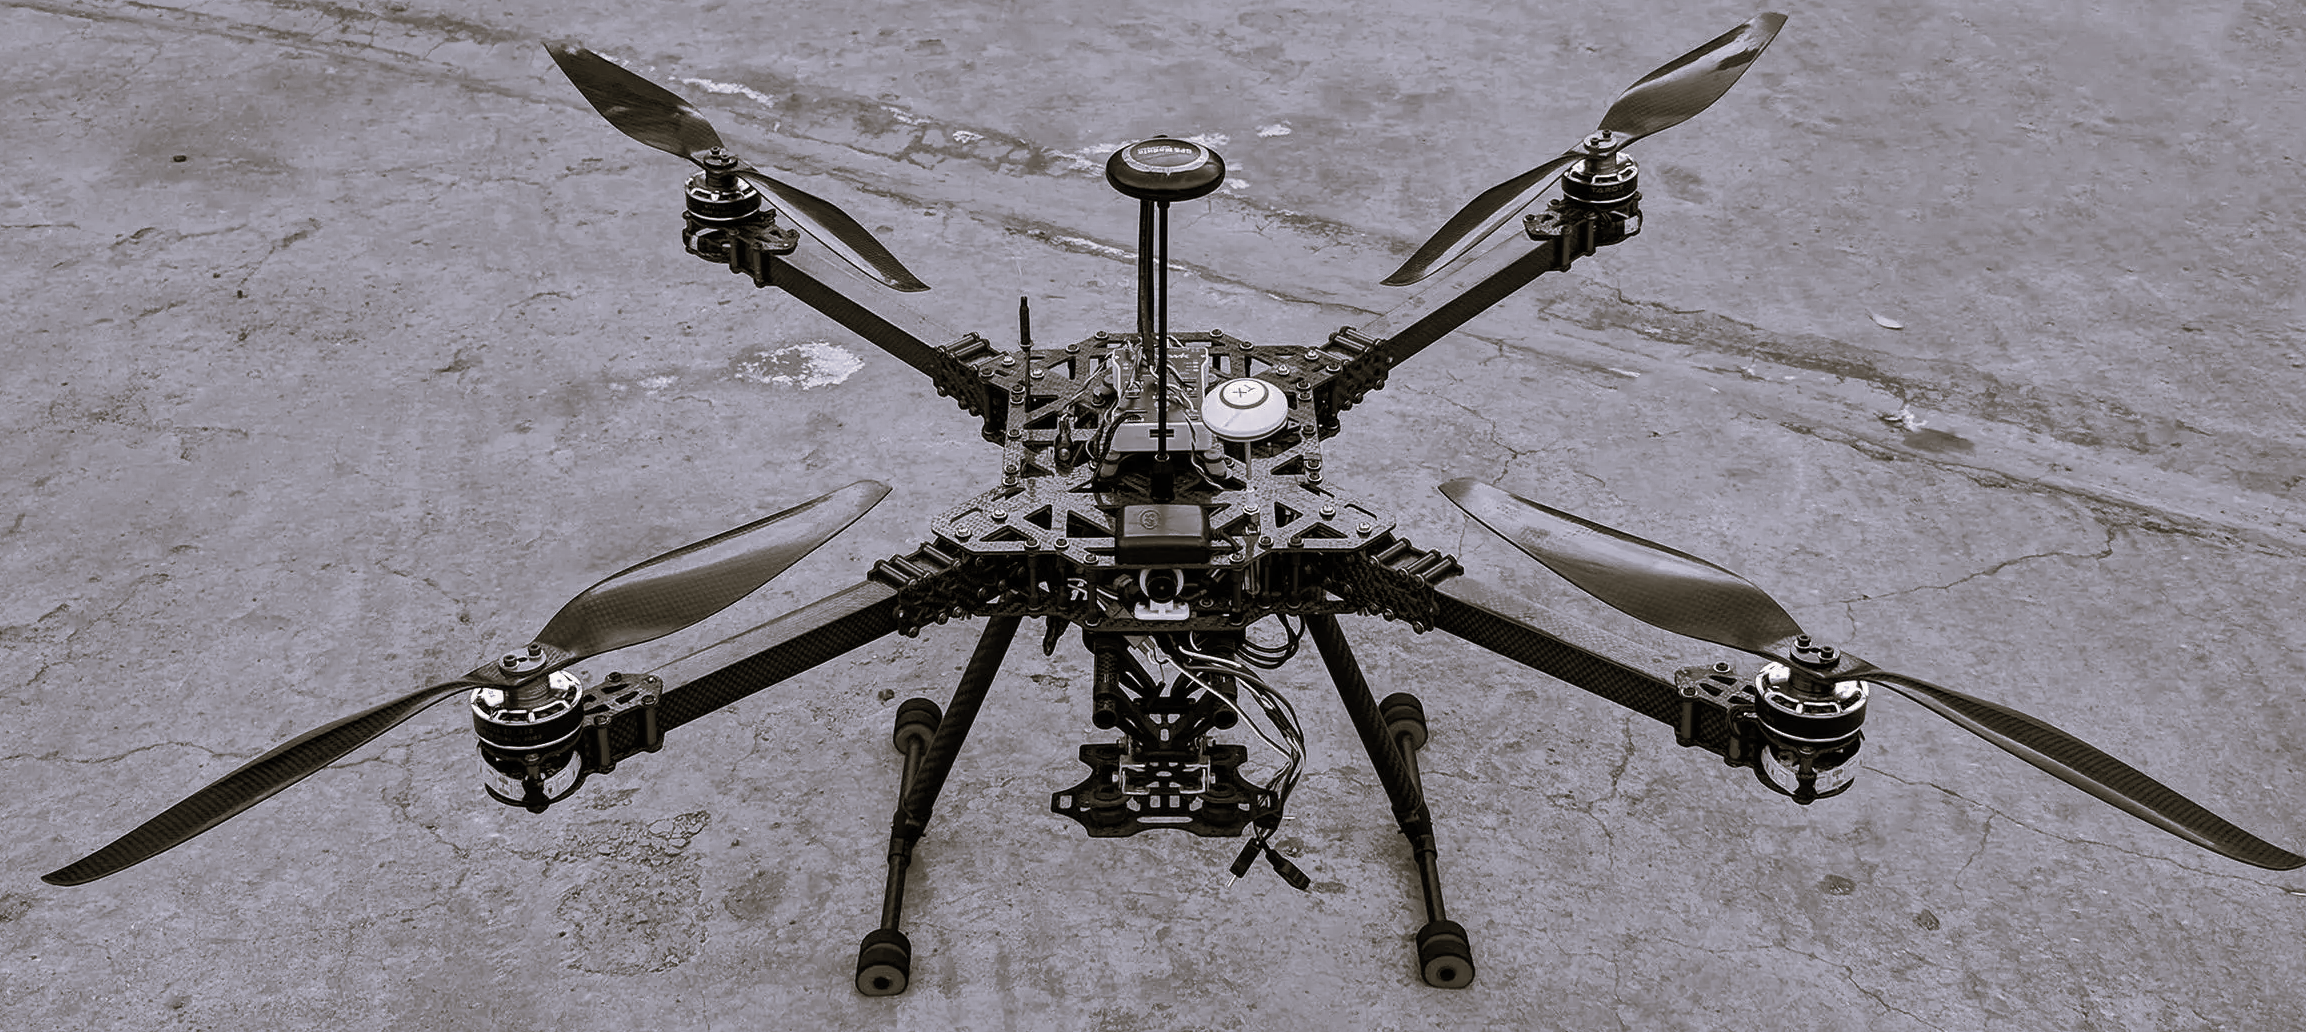
\includegraphics[width=\textwidth]{quadCopter.png}
\end{frame}


%% https://model-based-systems-engineering.com/2012/08/06/how-to-model-an-extended-system-context-with-sysml/
\begin{frame}
\frametitle {\textit{Mini} case study: a first model (II/II)}

\begin{figure}
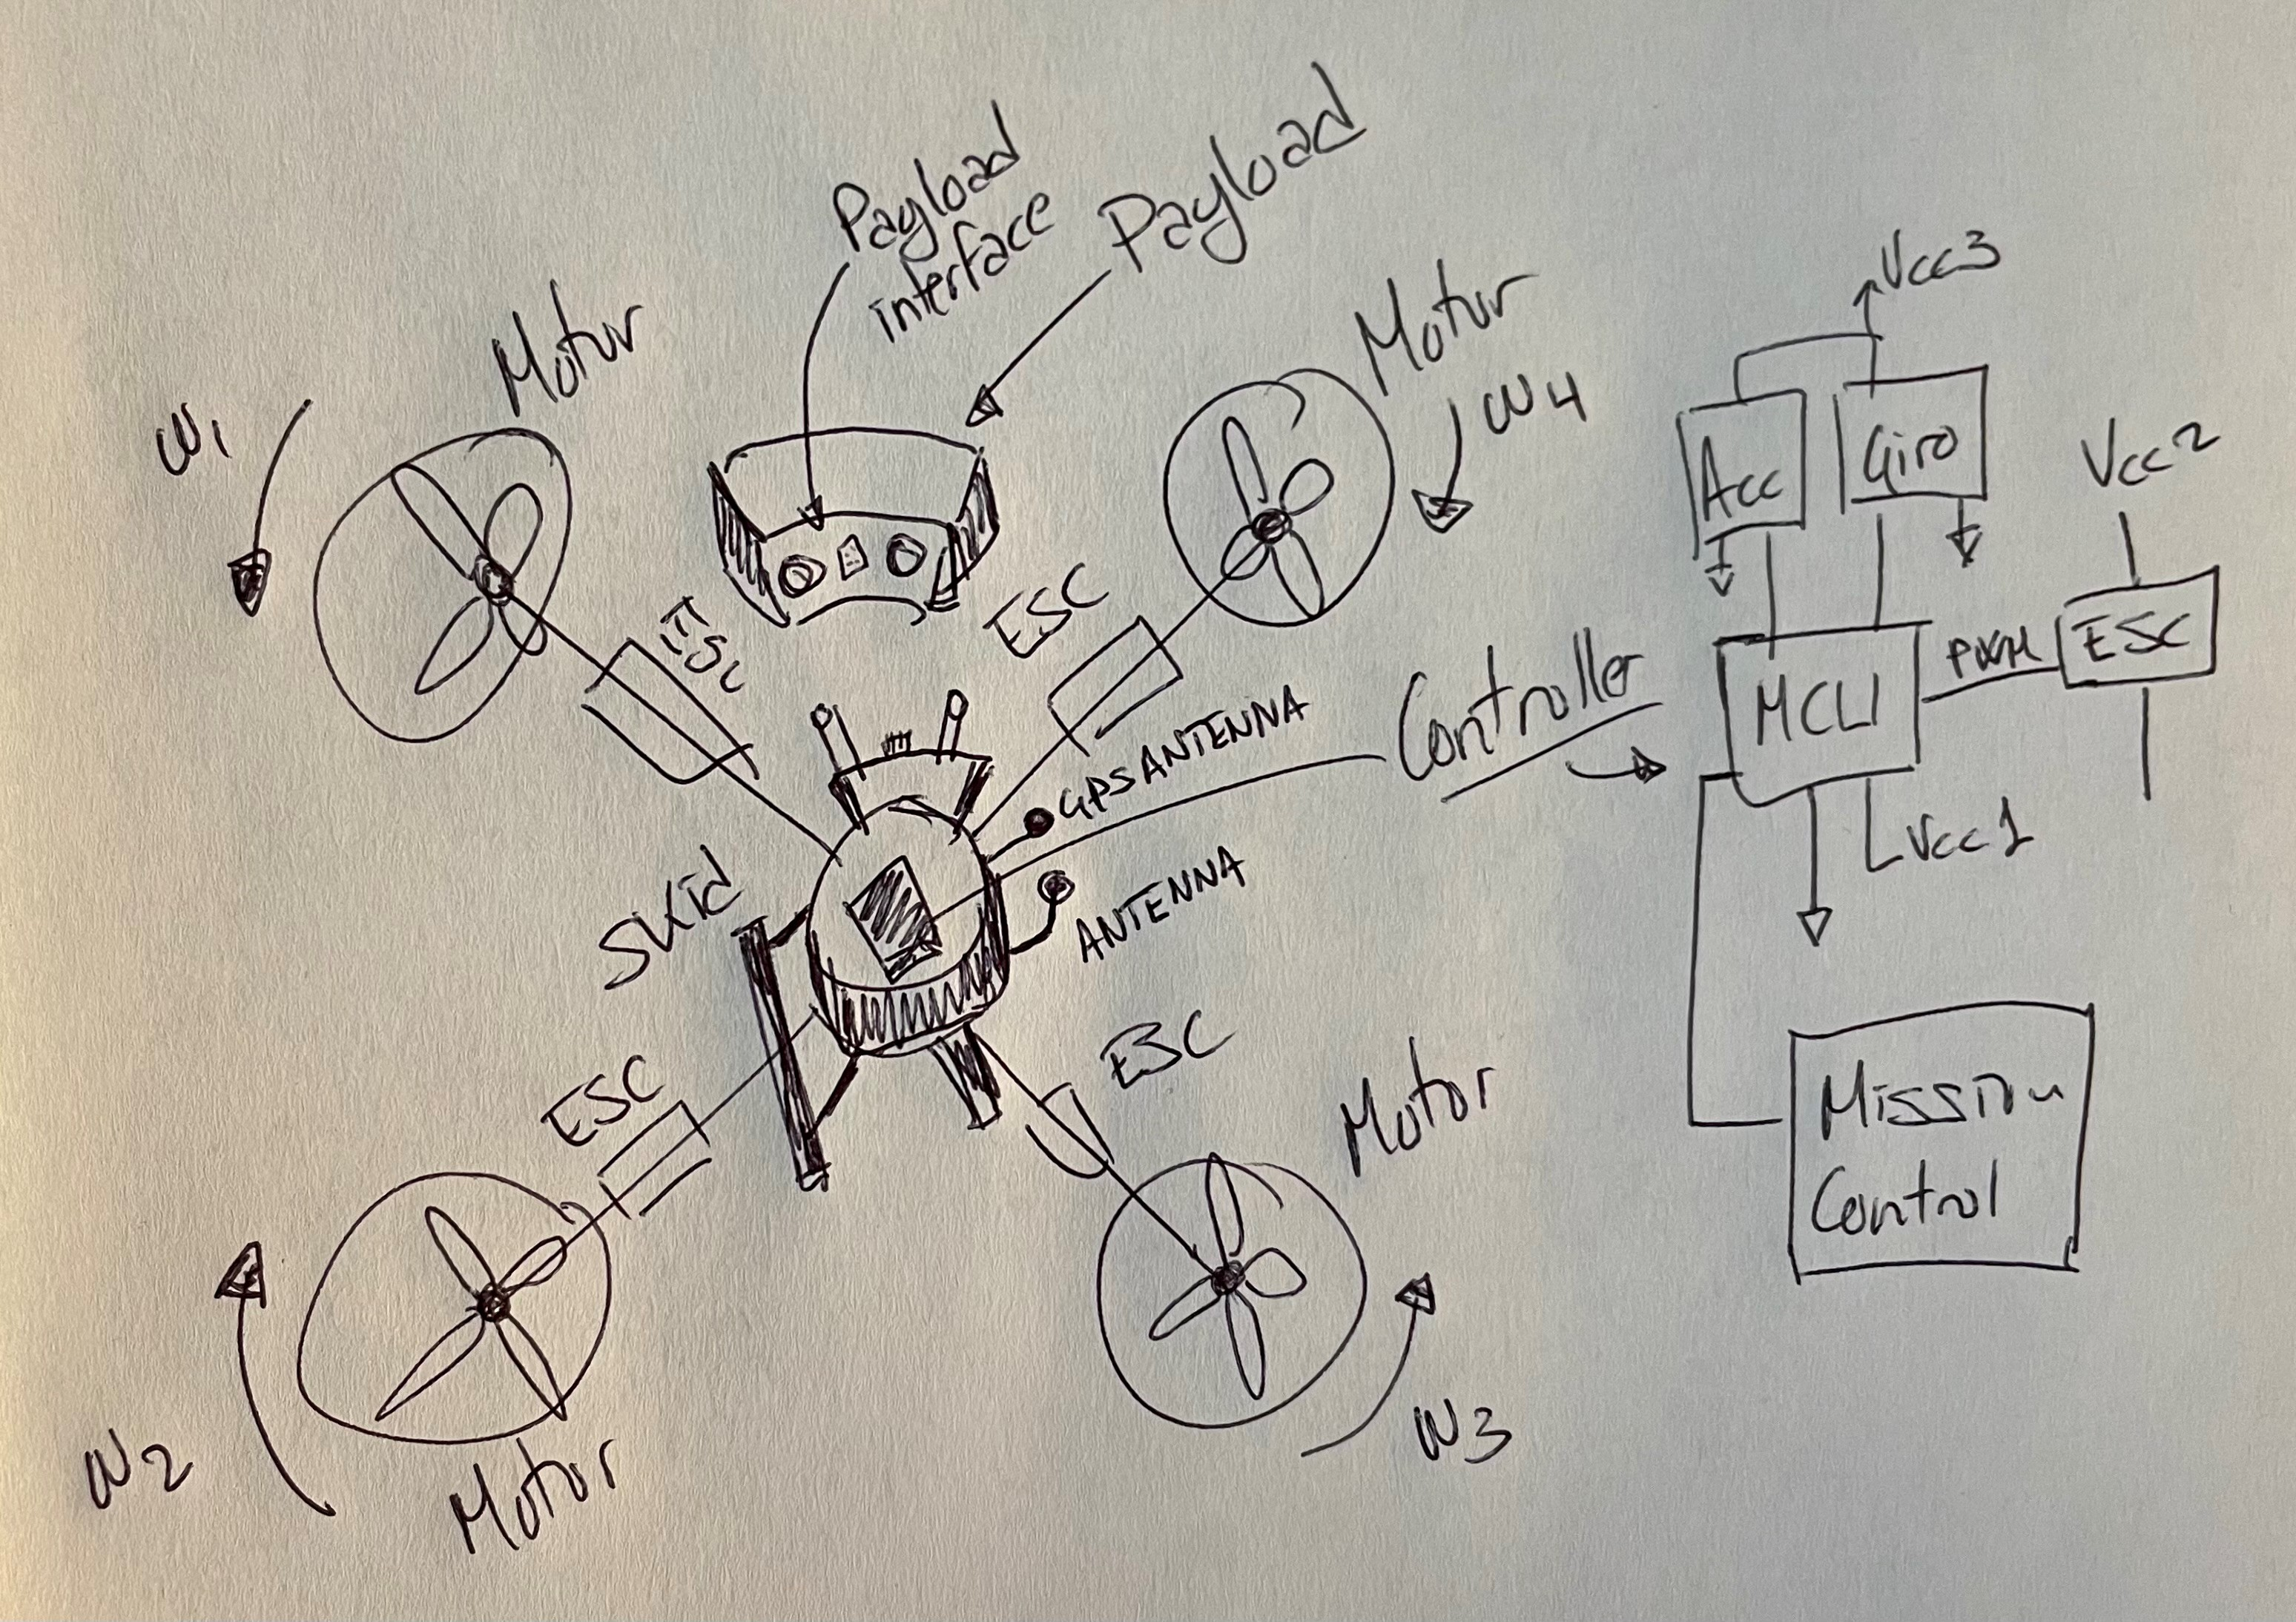
\includegraphics[width=0.7\textwidth]{quadModel1.jpg}
\end{figure}
\vspace{-5mm}


\begin{columns}

\begin{column}{0.5\textwidth}

\begin{itemize}
\small
\item  Do we have all structural elements?
\item Do we have a common level of abstraction?
\end{itemize}
\end{column}

\begin{column}{0.5\textwidth}

\begin{itemize}
\small
\item What does it mean to connect two blocks?
\item What is the model purpose?
\end{itemize}
\end{column}

\end{columns}


\end{frame}


\section{Modelling structure}
\subsection{Block Definition Diagrams}

\begin{frame}
\frametitle {Block Definition Diagram (BDD), structures and entities}
%%What is a block, what it can contain
We engineer entities, that have structure. They are composed of other entities. 
\begin{block}{}
%% Insert reference @TODO
%% difference between subject and object
%% examples for others
%{Entity definition (Wikipedia https://en.wikipedia.org/wiki/Entity )}
An entity is something that exists as itself, as a subject or as an object, actually or potentially, concretely or abstractly, physically or not. It does not need to be of material existence. Generally, there is no presumption that an entity is animate, or present.
% In particular, abstractions and legal fictions are usually regarded as entities. 
\end{block}

\begin{columns}

	\begin{column}{0.5\textwidth}
SysML \textbf{blocks} are entities, defined in BDD.
A block may have properties:
\begin{itemize}
\item Constituent \textbf{parts}.
\item \textbf{references} to parts that it uses.
\item \textbf{values} that characterize it.
\item \textbf{ports} to represent interfaces.
\item \textbf{operations} to represent behaviour.
\end{itemize}
	\end{column}

	\begin{column}{0.5\textwidth}
\vspace{-0.5cm}
\begin{figure}
 	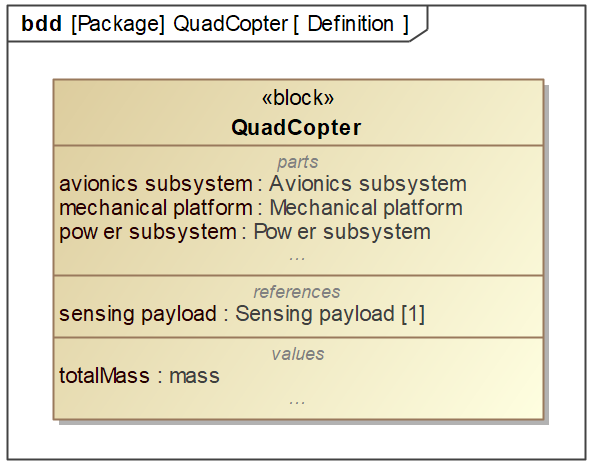
\includegraphics[width=0.8\textwidth]{BDD1.PNG}
\end{figure}
	\end{column}

%%TODO: missing to show an operation for the QuadCopter block

%% Here explain that the block has compartments
%% The system diagram is presented in a frame, with the definition
%% Blocks can be created at any level of abstraction

\end{columns}

\end{frame}

\begin{frame}
\frametitle{Relations between blocks (I/II)}
%% https://stackoverflow.com/questions/885937/what-is-the-difference-between-association-aggregation-and-composition
%% Relations between blocks, 
%% Explain multiplicity
\begin{itemize}
\item Composition: represents structural decomposition. It conveys ownership and hierarchy.% Composition aggregation, Composition association
\end{itemize}
\begin{figure}
 	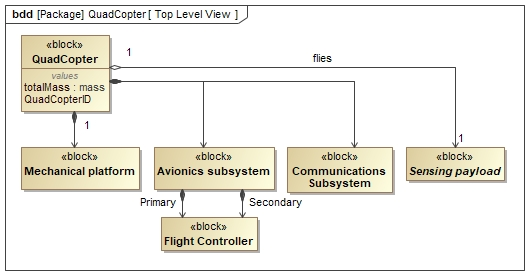
\includegraphics[width=0.7\textwidth]{QuadTopLevelView.jpg}
\end{figure}

%% In this example, a QuadCopter is composed of a mechanical platform, an avionics subsystem and a communications subsystem. Furthermore, the Avionics subsystem is composed of two Flight Controllers. The elements that are composing the quadcopter are all parts.

Elements that compose the QuadCopter are parts.\newline
Composition is represented using the black diamond.\newline
Multiplicity greater than two can also be represented discretely.

%% \footnotetext{Remember, 7 plus minus 2} 
%% https://en.wikipedia.org/wiki/The_Magical_Number_Seven,_Plus_or_Minus_Two and also mentioned Urwick 56 and incose handbook
%% Composition and connector examples can be found in page 72 in the standard.

%% \fixmegood{Add a short text elaborating a bit more on the composition, fix the multiplicity at the quadcopter side regarding the comm subsystem block}
\end{frame}

\begin{frame}
\frametitle{Relations between blocks (II/II)}
%% Association and relations used in requirements diagrams? Allocate and trace also.

%% The standard defines:
%%     - Reference Association (page 36)
%%     - Part Association (page 37)
%%     - Shared Association (page 37)
%% r

\begin{itemize}
\item Aggregation: represents a weaker relation than a composition, but still hierarchical.
\item Association: represents a connection between instances, similar to an aggregation, but without conveying the hierarchical facet.
\end{itemize}

Both are references. An instance can access the instance it refers. In general, a reference might be deleted, but the referred instance may still exist. % Reference property (shared aggregation).

%% \item Associations, %% Page 44 Can be used to represent the connection between blocks, especially when an entity is used to establish that connection. For example, a power cable.  The choice to use the references compartment notation versus reference associations depends on how much information you need to expose on the BDD.

%% Reference might be established through standard association or aggregation.

\begin{figure}
 	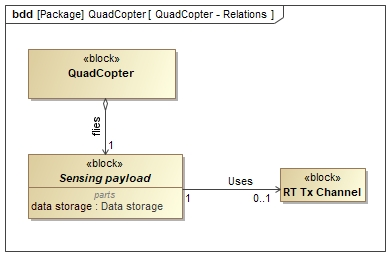
\includegraphics[width=0.5\textwidth]{QuadRelations.jpg}
\end{figure}

\end{frame}


\begin{frame}
\frametitle{Modelling multiplicity (I/II)}
\begin{itemize}
\item Relations can be specified in terms of multiplicity.
\item Multiplicity represents the number of instances that are a valid system representation.
\end{itemize}

\begin{figure}
 	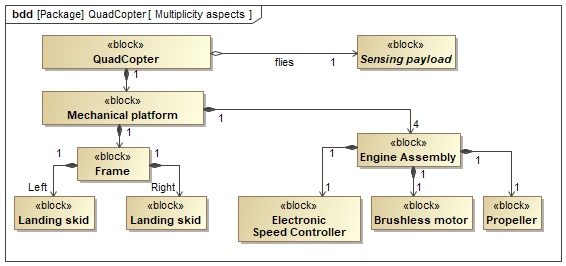
\includegraphics[width=0.7\textwidth]{QuadMultiplicity.jpg}
\end{figure}

\begin{itemize}
\item A mechanical platform is composed of four Engines Assemblies. An engine assembly composes only one mechanical platform.
\item A frame is composed of two Landing skids, named Left and Right. Each skid composes only one frame.
\end{itemize}

\end{frame}

\begin{frame}
\frametitle{Modelling multiplicity (II/II)}
\begin{itemize}
\item If no multiplicity is shown, the default applies.
\item In general, the default multiplicity is 1 to 1.
\item Composition and Aggregations have by default a multiplicity of [0..1] on the diamond end, making the reference or part optional.
\end{itemize}


Hard to believe, but that is how it is standardized:
\begin{figure}
 	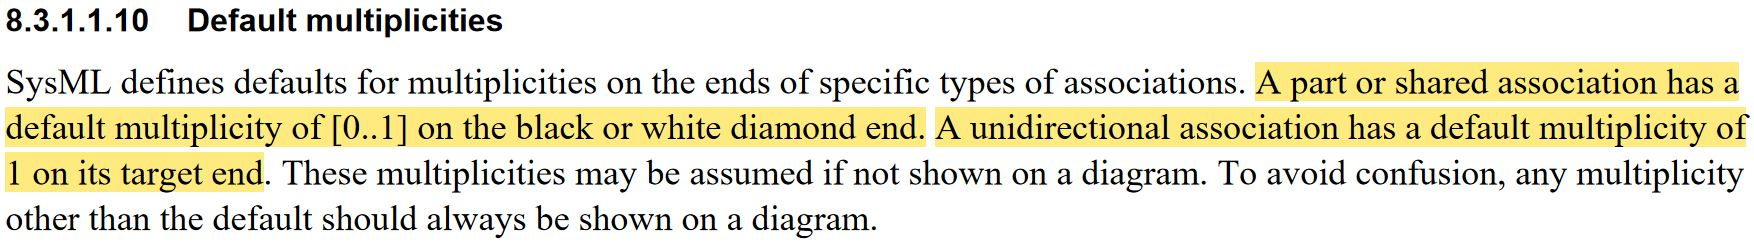
\includegraphics[width=0.9\textwidth]{MultiplicitiesStd.jpg}
\end{figure}

\begin{figure}
 	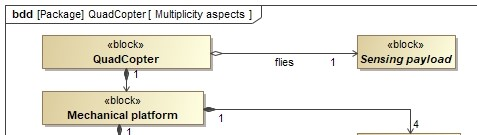
\includegraphics[width=0.5\textwidth]{QuadMultiplicityFocused.jpg}
\end{figure}

\end{frame}

\begin{frame}
\frametitle{Generalization (I/II)}
\begin{itemize}
\item It is typically used to model common aspects of a number of similar entities in one general block, called super-type.
\item The sub-types are specific blocks inheriting from the super-type, and extending it with specific properties.
\item The super-type, and part of its properties may be \textit{abstract}. An abstract block cannot be instantiated.
\end{itemize}

\begin{figure}
 	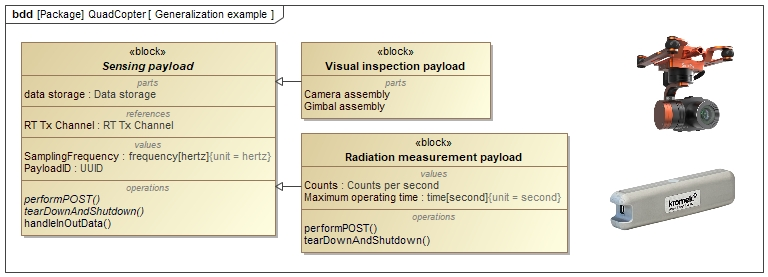
\includegraphics[width=\textwidth]{GeneralizationDetailed.jpg}
\end{figure}
\end{frame}




\begin{frame}
\frametitle{Generalization (II/II)}
\begin{figure}
 	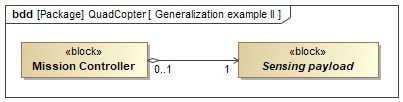
\includegraphics[width=0.6\textwidth]{GeneralizationExampleClient.jpg}
\end{figure}

\begin{itemize}
\item Provides a single point where changes can take place, without having to model them in all the sub-types individually.
\item A sub-type can replace a super-type in the model (Liskov substitution principle).
\item Other elements can also use generalization relations. E.g. Ports and interfaces.
\end{itemize}

Handle with care:\newline
\danger There might be several levels of inheritance.\newline
\danger A block might inherit from several blocks.
\end{frame}


\subsection{Ports}


%% Full ports vs proxy ports https://mbse4u.com/2013/09/23/sysml-full-ports-versus-proxy-ports/

\begin{frame}
\frametitle{Introduction to Ports}
\begin{itemize}
\item Entities that compose a system interact with each other.
\item SysML provides the \textbf{Port} property to specify interaction points.
\item Ports allow to show block boundaries and hide implementation aspects.
\end{itemize}

\vspace{-5mm}
\begin{columns}
\begin{column}{0.5\textwidth}
\begin{figure}
 	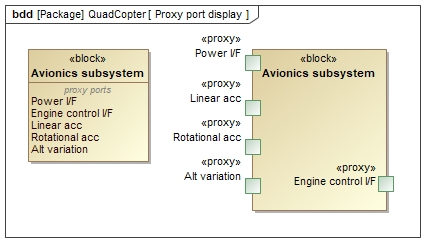
\includegraphics[width=\textwidth]{PortIntroductionI.jpg}
\end{figure}

\end{column}
\begin{column}{0.5\textwidth}
\begin{figure}
 	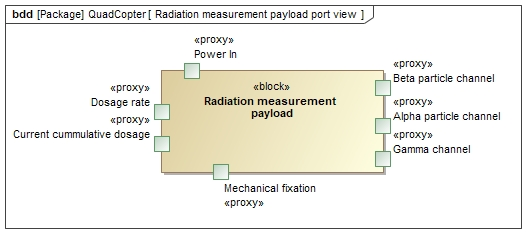
\includegraphics[width=\textwidth]{RadPayload.jpg}
\end{figure}
\end{column}
\end{columns}

\begin{itemize}
\item There are no constraints to what can flow, exchange or be provided through a port.
\item Ports can be used at the level of abstraction that is needed.
\end{itemize}

\end{frame}

% \item A port decouples the internals of a block from the client receiving a service, 
\vspace{-2mm}
\begin{frame}
\frametitle{Proxy Ports and interfaces}
\begin{itemize}
\item A proxy port exposes properties of its owning block. 
\item It is not an entity, has no properties of its own. It is an \textbf{access point}.
\item  It is typed by an interface.
\end{itemize}
\vspace{-2mm}
\begin{figure}
 	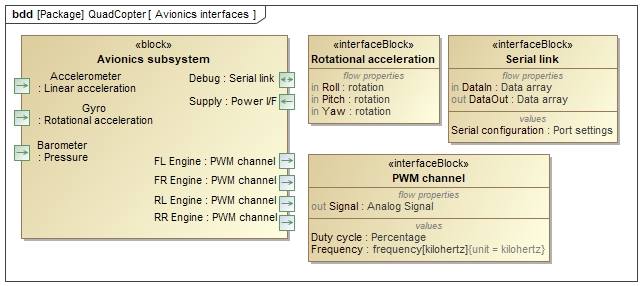
\includegraphics[width=0.8\textwidth]{QuadAvionicsInterfaces.jpg}
\end{figure}
%\begin{comment}
% 	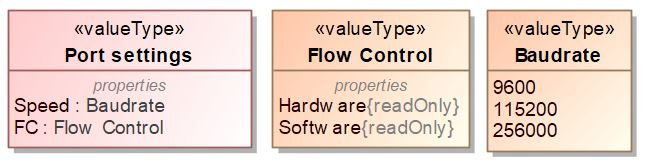
\includegraphics[width=0.5\textwidth]{PortInterfaceConfig.jpg}
%\end{comment}



\vspace{-9mm}
\begin{columns}
\begin{column}{0.5\textwidth}

\begin{itemize}
\item Value types can define values.
\item Proxy ports can be conjugated, reversing the direction of the flows.
%% \item Ranges and enumerations are supported
\end{itemize}
\end{column}

\begin{column}{0.5\textwidth}
\begin{figure}
 	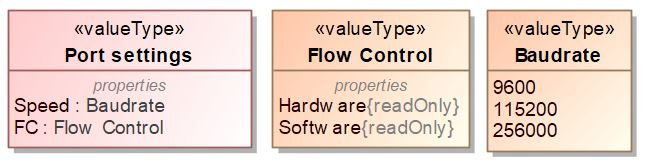
\includegraphics[width=\textwidth]{PortInterfaceConfig.jpg}
\end{figure}
\end{column}

\end{columns}
\end{frame}

\begin{frame}
\frametitle{Full Ports}

\begin{itemize}
\item It is an entity on its own. It is a part property of its owning block.
\item It is typed by a block $\longrightarrow$ it can have the same properties as a block.
%% Own properties, have internal structure, have behaviour.
\end{itemize}


\begin{figure}
 	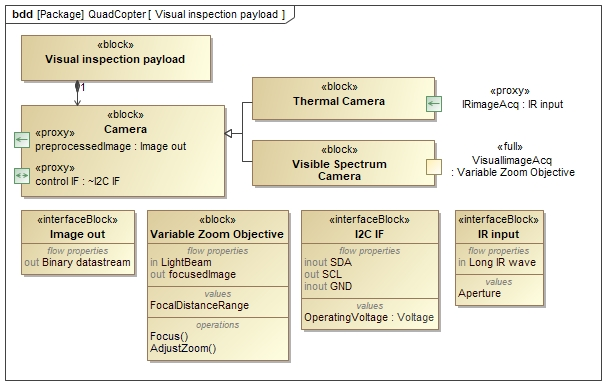
\includegraphics[width=0.8\textwidth]{VisualInspectionPayload.jpg}
\end{figure}



\end{frame}

\begin{frame}
\frametitle{Nested Ports}



\begin{itemize}
\item Ports can be nested, having several levels.
\item Nested ports allow to refine and detail further the interfaces.
\end{itemize}

\begin{figure}
 	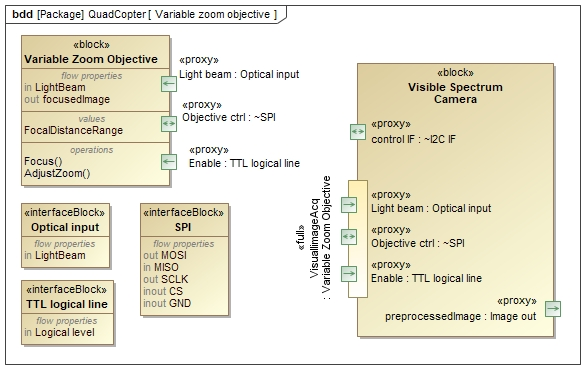
\includegraphics[width=0.8\textwidth]{PortsNested.jpg}
\end{figure}

%%\danger Think twice before nesting - Do not build ``towers'' of ports.
\end{frame}




\begin{comment}
\begin{frame}
\frametitle{Final words on Ports}
\begin{itemize}
\item As a general rule (I) favor proxy ports instead of full ports.
\item Avoid Flow ports, Flow specifications and Standard ports. Also lollipop/dot-socket notation. They are deprecated properties.
\end{itemize}
\end{frame}
\end{comment}


\subsection{Internal Block Diagrams}


\begin{frame}
\frametitle {Internal Block Diagrams (I/III)}
\begin{itemize}
\item IBDs display the internal structure of a block.
\item Connectors are used to display the relation between the block constituent parts and  also with their interfaces.
\item The interfaces can be external (ports at the block boundary) or internal (between constituent parts).
\end{itemize}
 %% SysML Distrilled, page 68 A connector between two properties on an IBD conveys that the two structures will have some way to access each other within a correctly assembled and operational system. It is not correct to consider connectors in the context of BDD. Connectors are elements used in IBDs.
%% \item References in IBD
%% \item Parts in IBD



\begin{columns}
\begin{column}{0.5\textwidth}
\begin{figure}
 	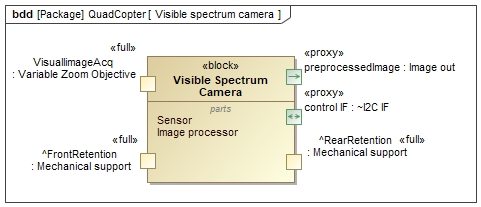
\includegraphics[width=\textwidth]{BDDVSCamera.jpg}
\end{figure}
\end{column}
\begin{column}{0.5\textwidth}
\begin{figure}
 	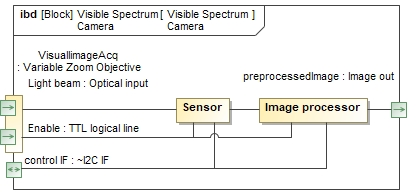
\includegraphics[width=\textwidth]{IBDVisibleSCamera.jpg}
\end{figure}
\end{column}


\end{columns}

\begin{itemize}
\item Parts can be connected directly, without using ports.
\end{itemize}
\end{frame}

\begin{frame}
\frametitle {Internal Block Diagrams (II/III)}

\begin{itemize}
\item Ports can be inherited through a generalization relation.	
\item Inherited ports are prepended with ``\textasciicircum''
\end{itemize}

\begin{columns}
	\begin{column}{0.4\textwidth}
		\begin{figure}
		 	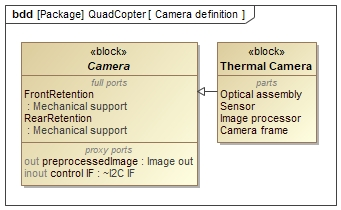
\includegraphics[width=\textwidth]{CameraAndThermalCam.jpg}
		\end{figure}
	\end{column}
	
	\begin{column}{0.6\textwidth}
		\begin{figure}
		 	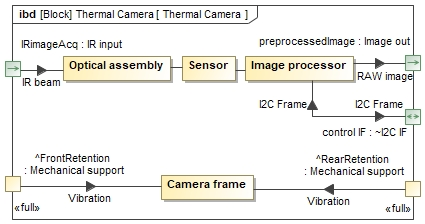
\includegraphics[width=0.9\textwidth]{IBDThermalCamera.jpg}
		\end{figure}
	\end{column}
\end{columns}

\begin{itemize}
\item Items can be added to illustrate item flows through connectors.
\end{itemize}

%% \fixmegood{Show as well that we can illustrate flows going through the connector}

\end{frame}


\begin{frame}
\frametitle{Internal Block Diagrams (III/III)}

\begin{itemize}
\item Blocks can be connected through ports at different levels of abstractions.
\item Internal structure can be displayed in a compartment within the block.
\item The binding connector, stereotyped \texttt{<<equal>>}, can be used to avoid having to repeat the port types.
\end{itemize}

\begin{figure}
    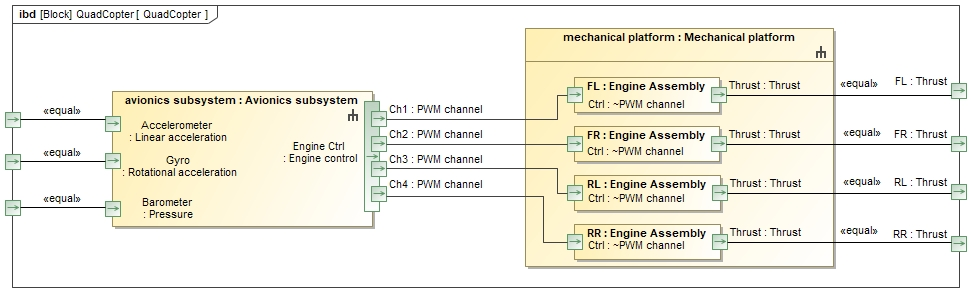
\includegraphics[width=\textwidth]{Composite.jpg}
\end{figure}
\end{frame}

\section{Concluding remarks}

\begin{frame}
\frametitle {Recapping}

In this presentation we have seen:
\begin{itemize}
\item How to model structural aspects of a system through BDD.
\item How to express hierarchy and interactions.
\item How to benefit from generalization for variability and maintainability.
\item How to model interfaces and interaction points.
\item How to model internal composition of Blocks through IBD.
\end{itemize}

With the modelling elements presented today one can navigate and understand more than 80\% of the models we have in Device HW.

\vspace{2mm}
\begin{block}{}
An entity is something that exists as itself, as a subject or as an object, actually or potentially, concretely or abstractly, physically or not. It does not need to be of material existence. Generally, there is no presumption that an entity is animate, or present.
% In particular, abstractions and legal fictions are usually regarded as entities. 
\end{block}

\end{frame}

\begin{frame}
\frametitle {Final words}
\begin{itemize}
\item This presentation had a strong focus on the language, its constructs and grammar.
\item Keep in mind that a perfectly constructed sentence can be absolute nonsense, and the same happens with models.
\end{itemize}

\textbf{Where to go from here?}
\begin{itemize}
\item Trainings on SysML organized by SET.
\item Start modelling, get feedback and model again.
\item Read and study material that I can share.
\item I can also prepare additional presentations with the same format focused on:
\begin{itemize}
\item Behavioral modelling
\item Good modelling practices
\item MagicDraw tool tutorials
\item All the above depending interests and FLSCs approval.
\end{itemize}
\end{itemize}

%%% SOLID applied to system modelling, interfaces.
%% Fan in fan out in components
%% 7+-2 principle
%% Professional Modelling tools vs. Drawing tools.
%% SysML 2

%% A very very good input on how to model interfaces and data flows
%% https://stackoverflow.com/questions/53011047/what-element-type-should-i-use-to-model-a-message-and-its-data-elements-in-sysml#53645147

%% https://en.wikipedia.org/wiki/SOLID
\end{frame}





\begin{comment}
Consider the relevance of SOLID in the context of modelling of systems with SysML
https://en.wikipedia.org/wiki/SOLID
\end{comment}

\end{document}